\documentclass[11pt,letterpaper]{article}
\usepackage[margin=0.75in]{geometry}
\usepackage[T1]{fontenc}
\usepackage{lmodern}
\usepackage{microtype}
\usepackage{graphicx}
\usepackage{booktabs}
\usepackage{tabularx}
\usepackage{array}
\usepackage{enumitem}
\usepackage{titlesec}
\usepackage{amssymb}
\usepackage{xurl}
\usepackage[hidelinks]{hyperref}
\usepackage{xcolor}

\setlist{nosep,leftmargin=1.2em}
\titleformat{\section}{\large\bfseries}{\thesection.}{0.5em}{}
\titlespacing*{\section}{0pt}{6pt}{2pt}
\setlength{\parindent}{0pt}
\setlength{\parskip}{3pt}
\newcolumntype{L}{>{\raggedright\arraybackslash}X}
\newcolumntype{P}[1]{>{\raggedright\arraybackslash}p{#1}}
\renewcommand{\arraystretch}{1.12}

\begin{document}

\begin{center}
{\Large\bfseries StudyLens: Graph-Grounded Diagram Understanding for Students}\\[3pt]
CECS 458/558 Term Project \textperiodcentered{} Phase 1: Integrated Ideation, Market Validation \& Feasibility Report\\[2pt]
\textbf{Krish Patel} \quad \textperiodcentered \quad October 16, 2026
\end{center}

StudyLens is a study assistant that answers student questions about diagrams by first extracting the diagram's entities and arrows into a graph, then answering from that graph with the supporting arrow highlighted. Phase 1 concludes the project is worth building: general AI assistants are documented to misread diagram relationships, public annotated data exists to measure this, and an open 3B-parameter model makes a working prototype feasible on one GPU within the course timeline.

\section{Industry and Target User}
\textbf{Industry:} Education technology, specifically AI-assisted self-study for STEM courses.
\textbf{Primary users:} undergraduate and advanced high-school students in diagram-heavy courses: introductory biology, chemistry, physics, earth science and computer science (flowcharts, network diagrams).
\textbf{Secondary users:} tutors and TAs who prepare practice material, and instructors.
\textbf{When the problem occurs:} a student studies alone, outside office hours, with a textbook figure or lecture slide they do not fully understand. They paste it into a general AI assistant and ask ``what feeds into X?''. The answer sounds confident, but the student cannot easily check whether it follows the arrows in the figure.

\section{Problem Definition}
\textbf{Pain point:} AI assistants identify the \emph{labels} in a diagram reliably but often get the \emph{arrows} wrong: what connects to what, in which direction, in what order. Students rarely notice, because the answer is fluent.
\textbf{Evidence:} Hou et al.\ [1] tested nine vision-language models (VLMs) on synthetic diagrams with no real-world knowledge to lean on. Entity recognition was near-perfect (87.5\% average; 99.2\% for GPT-4o). Recognizing explicit relations (arrows, lines) averaged only 58.9\%, and reasoning over them 52.6\%. Qwen2-2B, closest in size to our model, scored 44.0\% and 33.1\%. On a real food-web diagram, GPT-4o gave the same answer after every arrow was deleted or randomized. Its ``diagram reading'' was recall of biology facts.
\textbf{Consequences:} a reversed arrow in a pathway, circuit or flowchart is a conceptual error that students carry into exams. Errors are worst on unfamiliar or instructor-modified diagrams, exactly where help is needed. 
\textbf{Why it matters:} diagrams carry core content in every STEM course, and 92\% of students now study with AI [5]. A tool that answers from the figure itself, and shows its evidence, closes a gap that general assistants leave open.

\section{Proposed Solution and Main Workflow}
StudyLens is a web app that reads a diagram's \emph{structure} before answering. It builds an explicit graph of entities and directed relationships, answers from that graph and the image together, and points to the arrow that supports the answer. Workflow:
(1)~\textbf{Upload} a PNG/JPG figure, slide or flowchart;
(2)~\textbf{review} the extracted entities and arrows overlaid on the image (e.g., Sun$\rightarrow$Plant$\rightarrow$Rabbit);
(3)~\textbf{ask} a plain-language question (``Which component directly feeds into C?'');
(4)~\textbf{get a grounded answer} that cites the edges used (``B$\rightarrow$C''), highlights them, and abstains when no edge supports an answer;
(5)~\textbf{practice} with generated quiz questions whose answer key comes from the graph.
The differentiator is the visible, checkable middle step.

\section{AI Application Plan}
\textbf{Why AI rather than rules:} diagrams vary in style, arrow shape, icons and layout. Rule-based arrow detectors break on curved or crossing arrows, and free-form questions need language understanding.
\textbf{Why not end-to-end AI alone:} the evidence in \S2 shows end-to-end models fall back on memorized knowledge. We place checkable structure between perception and reasoning. A deterministic graph query answers structural questions (``what points to C?''), and the language model explains.

{\small
\begin{tabularx}{\textwidth}{@{}P{2.6cm}L@{}}
\toprule
\textbf{AI task} & Structured diagram parsing (entities + directed edges), then graph-grounded visual question answering and question generation \\
\textbf{Input} & Diagram image (PNG/JPG; later PDF pages) + natural-language question \\
\textbf{Intermediate} & JSON graph: nodes \{id, label, bbox, confidence\}; edges \{source, target, relation, confidence\} \\
\textbf{Output} & Answer + cited edges + highlighted regions; or a quiz with answer key \\
\textbf{Models} & Qwen2.5-VL-3B-Instruct [3] for extraction and answering (81.5 on AI2D; native bounding-box JSON); PaddleOCR [4] for labels; NetworkX for graph queries; PEFT/LoRA for optional fine-tuning \\
\bottomrule
\end{tabularx}}

\section{Initial Scope}
The MVP is one complete loop: upload a diagram, see its graph, ask, and get an answer with evidence. The research pipeline comes first; the app stays thin (single-page Next.js front end, FastAPI back end, one GPU).
\textbf{MVP (Phase 2):} image upload; entity/arrow extraction with overlay; graph-grounded Q\&A with highlighted evidence; experiment harness for E1--E3 on a fixed test split.
\textbf{Stretch:} quiz generation, student correction of wrong edges, LoRA fine-tuning (E4), PDF extraction, learning history.
\textbf{Out of scope:} handwritten notes, adaptive learning, multi-diagram reasoning.

\section{Market and Existing Solutions}
Students already study with AI and worry about accuracy. In HEPI's 2025 survey of 1,041 UK undergraduates, 92\% used AI tools (66\% in 2024), and 51\% said the risk of hallucinations puts them off [5]. IMARC sizes the AI-in-education market at USD 6.4B in 2025, forecasting 31\% annual growth to 2034 [6].

{\small
\begin{tabularx}{\textwidth}{@{}P{3.1cm}LLP{2.2cm}@{}}
\toprule
\textbf{Solution} & \textbf{What it does for diagrams} & \textbf{Gap StudyLens addresses} & \textbf{Price}\\
\midrule
ChatGPT Study Mode [7] & Accepts images; Socratic guidance and quizzes via prompting of the general model & Answers end-to-end, so exposed to knowledge shortcuts; no visible evidence & Free; paid tiers\\
Khanmigo [8] & AI tutor tied to Khan Academy content & Built around its own curriculum, not students' uploaded figures & \$4/mo; districts by quote\\
Quizlet AI [9] & Turns notes into flashcards and practice tests & Text-first; does not parse arrows or relations & Freemium\\
AI2D/DPG [2], Hou et al.\ [1] & Parse or benchmark diagram structure & Research, not student-facing products & Free (academic)\\
\bottomrule
\end{tabularx}}

\textbf{The gap:} general assistants cannot show \emph{which arrow} supports an answer, and study tools ignore the structure of figures. StudyLens combines both: it extracts the structure, answers from it, and shows the evidence.

\section{Business Feasibility}
StudyLens is viable as a low-cost study add-on, but only if Phase 3 shows a measurable accuracy gain over direct VLM answering. That gain is the value proposition.
\textbf{Value proposition:} ``answers about your diagram that you can check.'' Every answer cites its arrows, and it follows the instructor's actual figure, not the textbook version the model memorized.
\textbf{Expected users:} STEM undergraduates in introductory courses first, then AP/IB students, tutoring centres and TAs.
\textbf{Revenue:} (i)~freemium student subscription priced near Khanmigo's \$4/month, with a monthly diagram cap on the free tier; (ii)~per-seat institutional licences with LMS integration; (iii)~a per-call API for diagram-to-graph extraction for EdTech platforms and publishers.
\textbf{Cost:} self-hosted open-weight 3B--7B models on one GPU, with no per-token fee to a third-party API.
\textbf{Adoption barriers:} free incumbents (ChatGPT, Gemini) are ``good enough'' for many students; trust requires admitting uncertainty; institutions may restrict AI tools, so we position StudyLens as a study aid. Qwen2.5-VL-3B is research-licensed only [3], so a commercial launch needs the Apache-2.0 7B model. US school sales require FERPA-compliant data handling.

\section{Technical Approach}
We combine a VLM (computer vision), OCR and graph reasoning through an explicit intermediate representation. This fits the problem because the documented failure is in \emph{relations}, not \emph{entities}. We make relations explicit, measurable and checkable rather than hoping a larger model infers them.
\textbf{Research question:} does an extracted entity--relationship graph improve VLM accuracy on relationship questions about educational diagrams?

\begin{center}
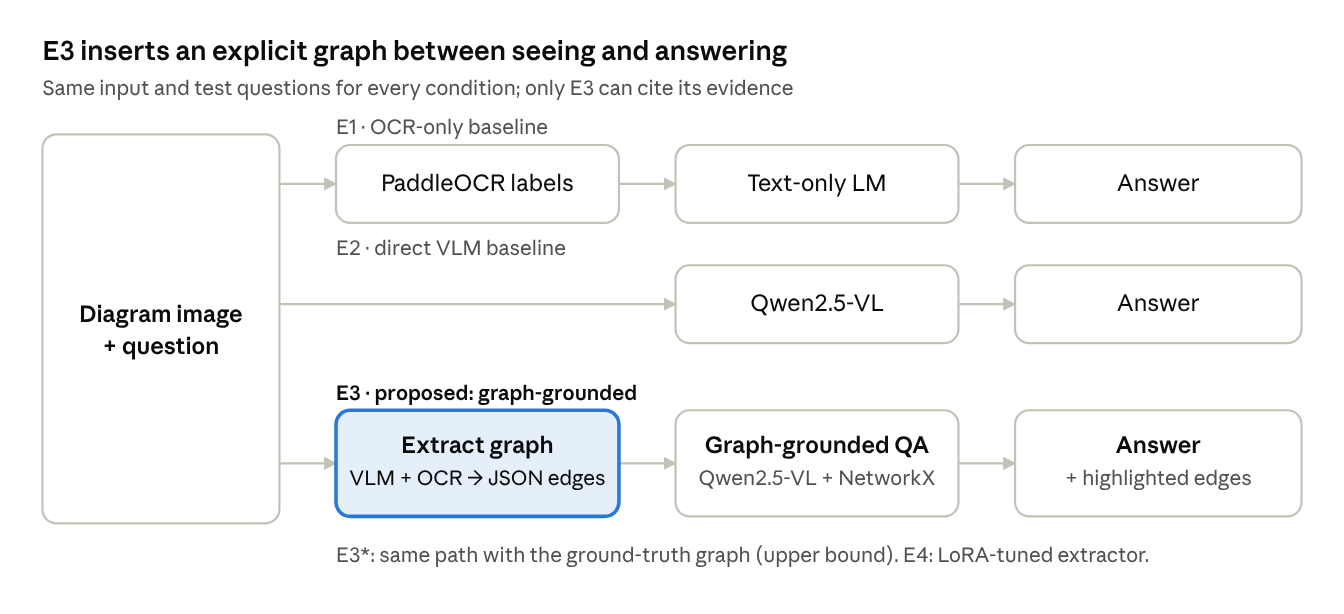
\includegraphics[width=0.72\textwidth]{figures/pipeline.png}\\[-2pt]
{\small\textbf{Figure 1.} Experimental conditions. E2 vs.\ E3 differ only in the graph step, so any gain is attributable to the explicit structure.}
\end{center}

\textbf{Conditions:} E1 OCR text only (lower baseline); E2 image + question to Qwen2.5-VL (main baseline); \textbf{E3 image + extracted graph (proposed)}; E3* ground-truth graph (upper bound, separating extraction from reasoning errors); E4 LoRA-tuned extractor (optional). Ablations remove OCR text, edges or coordinates from E3.
\textbf{Metrics:} \emph{primary} relationship-QA accuracy (E2 vs.\ E3, paired bootstrap 95\% CI on identical questions); entity F1, edge F1 and direction accuracy for extraction; hallucination rate (answers citing non-existent edges) and counterfactual consistency (does the answer change when an arrow is reversed?); latency per diagram.
\textbf{Known risk:} Hou et al.\ report that models given relations contradicting their prior knowledge tend to ignore them [1]. E3 therefore answers structural questions with a deterministic NetworkX query, and the counterfactual set tests whether the graph is actually followed.

\section{Data Plan}
\textbf{Preprocessing:} convert AI2D annotations to our JSON schema; normalize images; cache PaddleOCR output; tag each question as entity, relation or direction. We fix a seeded 70/10/20 split by diagram ID, and the test split never touches prompt tuning or LoRA training.
\textbf{Evaluation:} exact-match accuracy, entity/edge F1, and a 50-answer manual hallucination audit. A 20\% subset of the custom set is re-labelled after one week, and we report Cohen's $\kappa$.
\textbf{Privacy, bias, responsible use:} datasets contain no personal data. Prototype uploads are processed in memory and deleted at session end, and history is opt-in. No credentials go in the repo. AI2D is English-only and weighted to biology, so we add synthetic CS flowcharts and network diagrams.
\textbf{Fallback:} if AI2D conversion or annotation runs late, synthetic diagrams alone still answer E2 vs.\ E3 with exact labels.

{\small
\begin{tabularx}{\textwidth}{@{}P{2.5cm}LLL@{}}
\toprule
\textbf{Source} & \textbf{Content \& access} & \textbf{Licence / permission} & \textbf{Use}\\
\midrule
AI2D [2] & 4,903 grade-school science diagrams with annotated constituents and relationships; $>$15,000 multiple-choice questions; public download & Allen Institute terms (reported CC BY-SA; to confirm before redistribution) & Real-diagram QA; ground-truth graphs for E3* and edge F1\\
Hou et al.\ suite [1] & Generator for synthetic diagrams with known directed relations, plus evaluation code; public GitHub & No licence listed: evaluation use only, cited; authors contacted & Knowledge-free relation questions\\
Custom set (ours) & 150--200 diagrams: synthetic graphs + AI2D diagrams with arrows reversed or labels swapped & Ours; derivatives keep AI2D attribution & Counterfactual consistency, direction accuracy\\
\bottomrule
\end{tabularx}}

\section{Risks and Milestones}
{\small
\begin{tabularx}{\textwidth}{@{}P{5.2cm}P{1.5cm}L@{}}
\toprule
\textbf{Risk} & \textbf{Level} & \textbf{Mitigation}\\
\midrule
Extracted graphs have wrong or missing edges & High & Report edge F1 separately; E3* isolates the cause; OCR + boxes as extra cues\\
Model ignores a graph that contradicts its priors & Medium & Deterministic graph query; counterfactual test set\\
GPU time; slow annotation & Medium & 4-bit quantization, Colab/lab GPU, E4 as stretch; synthetic data gives exact labels\\
Confident wrong answers mislead students & Medium & Cite edges; abstain when no edge supports the answer\\
No advantage over free assistants & Medium & Phase 3 must show the E2$\rightarrow$E3 gain; pivot to API/B2B if consumer pull is weak\\
\bottomrule
\end{tabularx}}

\textbf{Milestones:} (1)~repo, data loaders, E1/E2 baselines on a 200-question pilot (\textbf{PoC gate}, Oct 30); (2)~graph extraction (VLM $\rightarrow$ JSON $\rightarrow$ NetworkX) and E3, Oct 31--Nov 13; (3)~FastAPI + Next.js upload $\rightarrow$ overlay $\rightarrow$ ask $\rightarrow$ highlighted answer, repo docs (\textbf{MVP gate}, Phase 2 report, Nov 20); (4)~counterfactual set, full test split, ablations, E3*, optional E4, Nov 21--Dec 4; (5)~failure analysis, demo video, final report (Dec 11).


\section*{References}
{\footnotesize
\begin{enumerate}[label={[\arabic*]},leftmargin=2em,itemsep=0pt]
\item Y.~Hou, B.~Giledereli, Y.~Tu, M.~Sachan. Do Vision-Language Models Really Understand Visual Language? \emph{ICML 2025}, PMLR 267:23910--23959. \url{https://proceedings.mlr.press/v267/hou25c.html}
\item A.~Kembhavi et al. A Diagram Is Worth a Dozen Images. \emph{ECCV 2016}. \url{https://arxiv.org/abs/1603.07396}
\item Qwen Team. Qwen2.5-VL-3B-Instruct model card and Qwen Research Licence. \url{https://huggingface.co/Qwen/Qwen2.5-VL-3B-Instruct}
\item PaddlePaddle. PaddleOCR (Apache-2.0). \url{https://github.com/PaddlePaddle/PaddleOCR}
\item Higher Education Policy Institute. Student Generative AI Survey 2025 (Feb 2025). \url{https://www.hepi.ac.uk/2025/02/26/student-generative-ai-survey-2025/}
\item IMARC Group. AI in Education Market Size, Share \& Growth Forecast 2034 (updated Oct 2026). \url{https://www.imarcgroup.com/ai-in-education-market}
\item AlternativeTo News. ChatGPT launches Study Mode (Jul 29, 2025). \url{https://alternativeto.net/news/2025/7/chatgpt-launches-study-mode-to-foster-student-learning-and-critical-thinking}
\item Khan Academy. Khanmigo pricing (accessed Oct 13, 2026). \url{https://khanmigo.ai/pricing}
\item Fortune Education. Quizlet's AI-powered tools (Oct 17, 2023). \url{https://fortune.com/education/articles/quizlet-ai-powered-tools-q-chat-magic-notes-quick-summary-gpt}
\end{enumerate}}

\end{document}
